\documentclass[12pt,a4paper]{article}

\usepackage{float}
\restylefloat{figure}
\usepackage{hyperref}
\usepackage{graphicx}
\usepackage{gensymb}
\usepackage[title]{appendix}
\usepackage[dotinlabels]{titletoc}
\usepackage[nottoc,numbib]{tocbibind}
\usepackage{mathtools}
\usepackage[margin=0.5in]{geometry}
\renewcommand{\thefootnote}{\arabic{footnote}}

\newcommand*\wrapletters[1]{\wr@pletters#1\@nil}
\def\wr@pletters#1#2\@nil{#1\allowbreak\if&#2&\else\wr@pletters#2\@nil\fi}

\usepackage{enumitem}
\setenumerate{itemsep=0pt}

% Add support for multi-page tables.
\usepackage{longtable}

\pagenumbering{arabic}

\title{EE4DSA Coursework 2}
\author{Chris Cummins}

\begin{document}
\maketitle

\section{Disassembling the program ROM}

The file \texttt{extra/rom.asm} contains a heavily annotated
disassembled version of the safe unlocking program, in a style
inspired by the AVR Assembler Syntax. The program tests for the safe
code 4D5A.

The assembly code was generated automatically using a disassembler
developed for this purpose, available at
\url{http://chriscummins.cc/disassembler}. Based off of the
implementation for the first coursework disassembler, the
functionality has been extended to support the subroutine and
interrupt instructions, and development effort has been focused on
making the output easier to understand.

Generated label names now distinguish between subroutines, interrupt
handlers and sections, and the UI now supports syntax highlighting,
automatic comment generation, line highlighting and jumping to
sections (clicking on a branch or jump instruction will now take the
user to the specific address).

\begin{figure}[H]
  \centering
  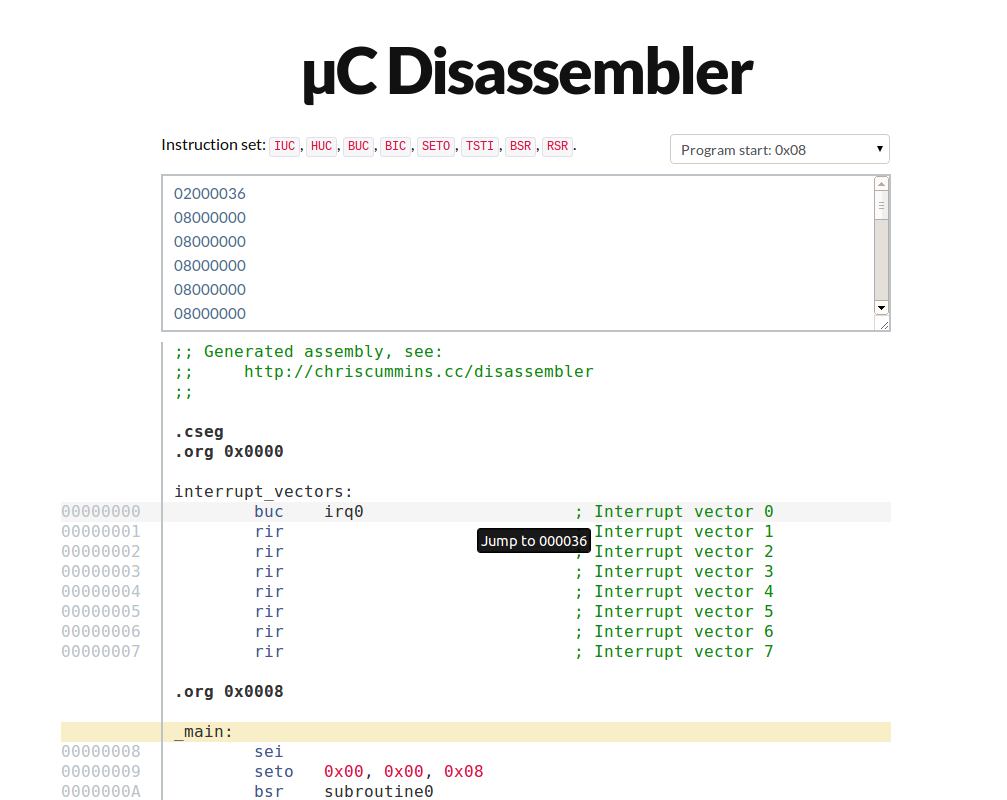
\includegraphics[width=6in]{assets/disassembler.png}
\end{figure}

The disassembler is implemented in JavaScript, with the source code
available at\\* \url{http://chriscummins.cc/js/disassembler.js}.

\section{Modifying the ROM program}

The file \texttt{rom.dat} contains a modified ROM program which uses
the last four digits of my SUN number (5189) as the code to the
safe. The only modifications required were to the \texttt{AND}
components of the four \texttt{TSTI} instructions. The
\texttt{test\_bench\_inputs.dat} file was then modified so as to test
this new code, and a process was added to the test bench program which
created a new \texttt{test\_bench\_outputs.dat} file.

\section{Implementing the Execution Unit}

The file \texttt{execution\_unit.vhd} contains my implementation of
the instruction set. In order to prevent warnings warnings during
synthesis about unused signals, assignments to test signals are
guarded with \texttt{--synopsys} directives. As a result, the program synthesises
without any pertinent warnings:

\begin{verbatim}
$ make synthesis
Synthesis running...
WARNING:Xst:2999 - Signal 'data', unconnected in block 'rom', is tied to its     \
 initial value.
WARNING:Xst:647 - Input <en> is never used. This port will be preserved and left \
 unconnected if it belongs to a top-level block or it belongs to a sub-block and \
 the hierarchy of this sub-block is preserved.
WARNING:Xst:2042 - Unit rom: 32 internal tristates are replaced by logic (pull-u \
 p yes): do<0>, do<10>, do<11>, do<12>, do<13>, do<14>, do<15>, do<16>, do<17>,  \
 do<18>, do<19>, do<1>, do<20>, do<21>, do<22>, do<23>, do<24>, do<25>, do<26>,  \
 do<27>, do<28>, do<29>, do<2>, do<30>, do<31>, do<3>, do<4>, do<5>, do<6>, do<7>\
 , do<8>, do<9>.5189
\end{verbatim}

A short video demonstrating the program can be found at
\url{http://youtu.be/KNiRIqV4vLQ}.

\end{document}
